% answers.tex —— 2000 年·上海卷·理科 · 参考答案与详细解析片段
% 由 tools/generate_projects.py 依来源总账自 2000/2000_数学真题_上海理_试题.md + 2000/2000_数学真题_上海理_解析正文.md + 2000/2000_数学真题_上海理_答案要点.md 生成，勿手改（改源 MD 后重跑）


\begin{gktip}
\textbf{来源说明}：固定 PDF 仅含题面，没有答案、解析或评分页。以下是本库独立推导，不是官方解析；出版者、版次、来源链及官方身份未核。Q12、Q21 的字面疑点保留 U/PENDING，不用常见题型或预期结果修订题面。
\end{gktip}

\gkpart{一、填空题}

\begin{answer}
\gksolhead{1}{}

\textbf{题目}：

已知向量 $\overrightarrow{OA}=(-1,2)$、$\overrightarrow{OB}=(3,m)$，若 $\overrightarrow{OA}\perp\overrightarrow{OB}$，则 $m=\underline{\qquad}$。

\Needspace{4\baselineskip}
\textbf{解析}

\Needspace{5\baselineskip}
由垂直向量的数量积为零，

\nopagebreak[4]
\[
(-1,2)\cdot(3,m)=-3+2m=0,
\]

所以 $m=\dfrac32$。

\gkanswer{答案：$m=\dfrac32$。}

\end{answer}
\begin{answer}
\gksolhead{2}{}

\textbf{题目}：

函数 $y=\log_{2}\dfrac{2x-1}{3-x}$ 的定义域为 $\underline{\qquad}$。

\Needspace{4\baselineskip}
\textbf{解析}

\Needspace{5\baselineskip}
对数真数必须为正：

\nopagebreak[4]
\[
\frac{2x-1}{3-x}>0.
\]

临界点为 $\dfrac12$ 与 $3$。作符号分析可知分式在两点之间为正，故定义域为 $\left(\dfrac12,3\right)$。

\gkanswer{答案：$\left(\dfrac12,3\right)$。}

\end{answer}
\begin{answer}
\gksolhead{3}{}

\textbf{题目}：

\Needspace{5\baselineskip}
圆锥曲线

\nopagebreak[4]
\[
\begin{cases}
x=4\sec\theta+1,\\
y=3\tan\theta,
\end{cases}
\]

的焦点坐标是 $\underline{\qquad}$。

\Needspace{4\baselineskip}
\textbf{解析}

\Needspace{5\baselineskip}
由 $\sec^2\theta-\tan^2\theta=1$ 消去参数，得到

\nopagebreak[4]
\[
\frac{(x-1)^2}{16}-\frac{y^2}{9}=1.
\]

这是中心为 $(1,0)$ 的双曲线，$a^2=16$、$b^2=9$，故 $c=\sqrt{a^2+b^2}=5$。焦点为 $(-4,0)$ 与 $(6,0)$。

\gkanswer{答案：焦点为 $(-4,0)$、$(6,0)$。}

\end{answer}
\begin{answer}
\gksolhead{4}{}

\textbf{题目}：

计算：$\displaystyle\lim_{n\to\infty}\left(\dfrac{n}{n+2}\right)^n=\underline{\qquad}$。

\Needspace{4\baselineskip}
\textbf{解析}

\nopagebreak[4]
\[
\left(\frac{n}{n+2}\right)^n=\left(1+\frac2n\right)^{-n}\longrightarrow e^{-2}.
\]

\gkanswer{答案：$e^{-2}$。}

\end{answer}
\begin{answer}
\gksolhead{5}{}

\textbf{题目}：

已知 $f(x)=2^x+b$ 的反函数为 $f^{-1}(x)$，若 $y=f^{-1}(x)$ 的图象经过点 $Q(5,2)$，则 $b=\underline{\qquad}$。

\Needspace{4\baselineskip}
\textbf{解析}

反函数图象经过 $(5,2)$，等价于原函数图象经过交换坐标所得的点 $(2,5)$，所以 $f(2)=5$。代入 $f(x)=2^x+b$ 得 $4+b=5$，故 $b=1$。

\gkanswer{答案：$b=1$。}

\end{answer}
\begin{answer}
\gksolhead{6}{}

\textbf{题目}：

根据上海市人大十一届三次会议上的市政府工作报告，1999 年上海市完成 GDP（GDP 是指国内生产总值）4035 亿元，2000 年上海市 GDP 预期增长 9\%，市委、市府提出本市常住人口每年的自然增长率将控制在 0.08\%，若 GDP 与人口均按这样的速度增长，则要使本市年人均 GDP 达到或超过 1999 年的 2 倍，至少需 $\underline{\qquad}$ 年。

按：1999 年本市常住人口总数约 1300 万。

\Needspace{4\baselineskip}
\textbf{解析}

\Needspace{5\baselineskip}
设经过 $n$ 年。GDP 和人口每年的增长因子分别为 $1.09$、$1.0008$，故人均 GDP 的年度增长因子为 $1.09/1.0008$。满足

\nopagebreak[4]
\[
\left(\frac{1.09}{1.0008}\right)^n\geq2
\quad\Longleftrightarrow\quad
n\geq\frac{\ln2}{\ln(1.09/1.0008)}\approx8.11857.
\]

因此至少需 $9$ 年。

\gkanswer{答案：至少 $9$ 年。}

\end{answer}
\begin{answer}
\gksolhead{7}{}

\textbf{题目}：

命题 A：底面为正三角形，且顶点在底面的射影为底面中心的三棱锥是正三棱锥，命题 A 的等价题 B 可以是：底面为正三角形，且 $\underline{\qquad}$ 的三棱锥是正三棱锥。

\Needspace{4\baselineskip}
\textbf{解析}

若顶点在底面中心正上方，顶点到底面三个顶点的距离相等。反过来，若三条侧棱相等，则顶点在底面上的射影到正三角形三个顶点等距；该射影只能是正三角形中心。因此可将条件改写为“三条侧棱相等”。

\gkanswer{答案：可填“三条侧棱相等”。}

\end{answer}
\begin{answer}
\gksolhead{8}{}

\textbf{题目}：

设函数 $y=f(x)$ 是最小正周期为 2 的偶函数，它在区间 $[0,1]$ 上的图象为如图所示的线段 $AB$，则在区间 $[1,2]$ 上 $f(x)=\underline{\qquad}$。
\nopagebreak[4]
\begin{center}% Generator: hand-authored TikZ from the source-visible axes, segment, and labels.
% Source: src-b46bf909434f6686413681f206c6f1c3566760d6e574f4799dc8b1e0658f9ee8
% PDF SHA-256: b798af61afdac624589769db5bbafe734aa9a0016973bd00b3f5bc8028ab3a40
% PDF page 1, printed page 70, question 8. Only the printed segment and labels are shown.
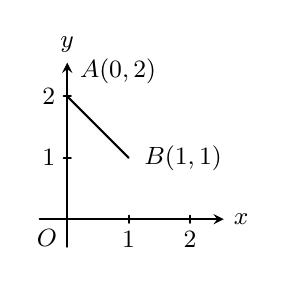
\begin{tikzpicture}[x=0.78cm,y=0.78cm,line cap=round,line join=round,line width=0.65pt,>=stealth,font=\small]
  \draw[->] (-0.45,0) -- (2.55,0) node[right] {$x$};
  \draw[->] (0,-0.45) -- (0,2.55) node[above] {$y$};
  \draw (-0.06,1) -- (0.06,1) node[left=2pt] {$1$};
  \draw (-0.06,2) -- (0.06,2) node[left=2pt] {$2$};
  \draw (1,-0.06) -- (1,0.06) node[below=2pt] {$1$};
  \draw (2,-0.06) -- (2,0.06) node[below=2pt] {$2$};
  \node[below left] at (0,0) {$O$};
  \draw[thick] (0,2) -- (1,1);
  \node[above right=1pt] at (0,2) {$A(0,2)$};
  \node[right=2pt] at (1,1) {$B(1,1)$};
\end{tikzpicture}
\end{center}
\nopagebreak[4]
\Needspace{4\baselineskip}
\textbf{解析}

\Needspace{5\baselineskip}
线段端点为 $A(0,2)$、$B(1,1)$，故 $0\leq t\leq1$ 时 $f(t)=2-t$。当 $1\leq x\leq2$ 时，周期性给出 $f(x)=f(x-2)$，偶性给出 $f(x-2)=f(2-x)$，从而

\nopagebreak[4]
\[
f(x)=2-(2-x)=x.
\]

\gkanswer{答案：$f(x)=x$（$1\leq x\leq2$）。}

\end{answer}
\begin{answer}
\gksolhead{9}{}

\textbf{题目}：

在二项式 $(x-1)^{11}$ 的展开式中，系数最小的项的系数为 $\underline{\qquad}$。（结果用数值表示）

\Needspace{4\baselineskip}
\textbf{解析}

$(x-1)^{11}$ 的一般项系数为 $(-1)^k\binom{11}{k}$。最大二项式系数为 $\binom{11}{5}=\binom{11}{6}=462$；$k=5$ 时符号为负，故最小系数为 $-462$。

\gkanswer{答案：$-462$。}

\end{answer}
\begin{answer}
\gksolhead{10}{}

\textbf{题目}：

有红、黄、蓝三种颜色的旗帜各 3 面，在每种颜色的 3 面旗帜上分别标上号码 1、2 和 3，现任取出 3 面，它们的颜色与号码均不相同的概率是 $\underline{\qquad}$。

\Needspace{4\baselineskip}
\textbf{解析}

总取法数为 $\binom93=84$。颜色和号码均各不相同，意味着每种颜色取一面且号码 $1,2,3$ 各出现一次，共有 $3!=6$ 种有利取法。因此概率为 $6/84=1/14$。

\gkanswer{答案：$\dfrac1{14}$。}

\end{answer}
\begin{answer}
\gksolhead{11}{}

\textbf{题目}：

在极坐标系中，若过点 $(3,0)$ 且与极轴垂直的直线交曲线 $\rho=4\cos\theta$ 于 $A\text{、}B$ 两点，则 $|AB|=\underline{\qquad}$。

\Needspace{4\baselineskip}
\textbf{解析}

由 $\rho=4\cos\theta$ 及 $x=\rho\cos\theta$、$y=\rho\sin\theta$，得 $x^2+y^2=4x$，即 $(x-2)^2+y^2=4$。过 $(3,0)$ 且垂直极轴的直线为 $x=3$，交点满足 $y^2=3$，故弦长 $|AB|=2\sqrt3$。

\gkanswer{答案：$2\sqrt3$。}

\end{answer}
\begin{answer}
\gksolhead{12}{}

\textbf{题目}：

\Needspace{5\baselineskip}
在等差数列 $\{a_n\}$ 中，若 $a_{10}=0$，则有等式

\nopagebreak[4]
\[
a_1+a_2+\cdots+a_n=a_1+a_2+\cdots+a_{19-n}\quad(n<19,\ n\in\mathbb{N}^{*})
\]

成立，类比上述性质，相应地：在等此数列 $\{b_n\}$ 中，若 $b_9=1$，则有等式 $\underline{\qquad}$ 成立。

\begin{gktip}
原页在“等此数列”中该字经 300 dpi 局部放大辨认为“此”。此处语义异常，可能涉及原卷印字或来源文字问题；本稿照录并标为待核，不代改为“等比”。
\end{gktip}

\Needspace{4\baselineskip}
\textbf{解析}

原页字面为“等此数列”，无法确认所指数列类型，标记 \textbf{U/PENDING}；因此本题不定稿答案。

\Needspace{5\baselineskip}
仅作条件性演算：若有可靠同版材料证明此处应为“等比数列”，设公比为 $q$。由 $b_9=1$ 得 $b_j=q^{j-9}$，于是

\nopagebreak[4]
\[
b_1b_2\cdots b_n=q^{\sum_{j=1}^{n}(j-9)}=q^{n(n-17)/2}.
\]

\Needspace{5\baselineskip}
令 $m=17-n$，则

\nopagebreak[4]
\[
b_1b_2\cdots b_{17-n}
=q^{\sum_{j=1}^{17-n}(j-9)}
=q^{(17-n)(-n)/2}
=q^{n(n-17)/2}.
\]

所以在该假设下，两边乘积相等（$1\leq n<17$）。这不构成对原卷字样的裁定，不能列为确定答案。

\gkanswer{答案：U/PENDING。}

\end{answer}
\gkpart{二、选择题}

\begin{answer}
\gksolhead{13}{}

\textbf{题目}：

复数 $z=-3\left(\cos\dfrac{\pi}{5}-i\sin\dfrac{\pi}{5}\right)$（$i$ 是虚数单位）的三角形式是\mbox{（　　）}。

（A）$3\left[\cos\left(-\dfrac{\pi}{5}\right)+i\sin\left(-\dfrac{\pi}{5}\right)\right]$

（B）$3\left(\cos\dfrac{\pi}{5}+i\sin\dfrac{\pi}{5}\right)$

（C）$3\left(\cos\dfrac{4\pi}{5}+i\sin\dfrac{4\pi}{5}\right)$

（D）$3\left(\cos\dfrac{6\pi}{5}-i\sin\dfrac{6\pi}{5}\right)$

\Needspace{4\baselineskip}
\textbf{解析}

负号可并入辐角：$-\operatorname{cis}(-\pi/5)=\operatorname{cis}(4\pi/5)$。故题给复数为 $3(\cos\frac{4\pi}5+i\sin\frac{4\pi}5)$，选（C）。

\gkanswer{答案：C。}

\end{answer}
\begin{answer}
\gksolhead{14}{}

\textbf{题目}：

设有不同的直线 $a$、$b$ 和不同的平面 $\alpha$、$\beta$、$\gamma$，给出下列三个命题：

① 若 $a\parallel\alpha$，$b\parallel\alpha$，则 $a\parallel b$；

② 若 $a\parallel\alpha$，$a\parallel\beta$，则 $\alpha\parallel\beta$；

③ 若 $\alpha\perp\gamma$，$\beta\perp\gamma$，则 $\alpha\parallel\beta$。

其中正确的个数是\mbox{（　　）}。

（A）0　　（B）1　　（C）2　　（D）3

\Needspace{4\baselineskip}
\textbf{解析}

三个命题均不成立。① 同一平面上方可取两条相交直线，它们都平行于该平面但彼此不平行。② 直线可平行于两个相交平面，例如方向平行于两平面的交线且位置不与平面相交。③ 两个平面可同时垂直于同一平面而彼此相交。因此正确个数为 $0$，选（A）。

\gkanswer{答案：A（正确命题个数为 $0$）。}

\end{answer}
\begin{answer}
\gksolhead{15}{}

\textbf{题目}：

若集合 $S=\{y\mid y=3^x,\ x\in\mathbb{R}\}$，$T=\{y\mid y=x^2-1,\ x\in\mathbb{R}\}$，则 $S\cap T$ 是\mbox{（　　）}。

（A）$S$　　（B）$T$　　（C）$\varnothing$　　（D）有限集

\Needspace{4\baselineskip}
\textbf{解析}

$S$ 是 $3^x$ 的值域，即 $(0,+\infty)$；$T$ 是 $x^2-1$ 的值域，即 $[-1,+\infty)$。故 $S\cap T=S$，选（A）。

\gkanswer{答案：A（$S\cap T=S$）。}

\end{answer}
\begin{answer}
\gksolhead{16}{}

\textbf{题目}：

下列命题中正确的命题是\mbox{（　　）}。

（A）若点 $P(a,2a)$（$a\ne0$）为角 $\alpha$ 终边上一点，则 $\sin\alpha=\dfrac{2\sqrt5}{5}$。

（B）同时满足 $\sin\alpha=\dfrac12$，$\cos\alpha=\dfrac{\sqrt3}{2}$ 的角 $\alpha$ 有且只有一个。

（C）当 $|a|<1$ 时，$\tan(\arcsin a)$ 的值恒正。

（D）三角方程 $\tan\left(x+\dfrac{\pi}{3}\right)=\sqrt3$ 的解集为 $\{x\mid x=k\pi,\ k\in\mathbb{Z}\}$。

\Needspace{4\baselineskip}
\textbf{解析}

\Needspace{5\baselineskip}
（A）中 $\sin\alpha=2a/(\sqrt5|a|)$，随 $a$ 的正负改变；（B）中的角可相差 $2k\pi$；（C）中 $\tan(\arcsin a)=a/\sqrt{1-a^2}$，不恒为正。只有（D）正确：

\nopagebreak[4]
\[
\tan\left(x+\frac\pi3\right)=\sqrt3
\Longleftrightarrow
x+\frac\pi3=\frac\pi3+k\pi
\Longleftrightarrow x=k\pi.
\]

\gkanswer{答案：D（解集为 $\{x\mid x=k\pi,\ k\in\mathbb Z\}$）。}

\end{answer}
\gkpart{三、解答题}

\begin{answer}
\gksolhead{17}{}

\textbf{题目}：

已知椭圆 $C$ 的焦点分别为 $F_1(-2\sqrt2,0)$ 和 $F_2(2\sqrt2,0)$，长轴长为 6，设直线 $y=x+2$ 交椭圆 $C$ 于 $A\text{、}B$ 两点，求线段 $AB$ 的中点坐标。

\Needspace{4\baselineskip}
\textbf{解析}

\Needspace{5\baselineskip}
椭圆半长轴 $a=3$，焦距参数 $c=2\sqrt2$，故 $b^2=a^2-c^2=1$，方程为 $x^2/9+y^2=1$。代入直线 $y=x+2$，得

\nopagebreak[4]
\[
10x^2+36x+27=0.
\]

两交点横坐标之和为 $-36/10=-18/5$，中点横坐标为 $-9/5$。直线上的纵坐标为横坐标加 $2$，故中点为 $\left(-\dfrac95,\dfrac15\right)$。

\gkanswer{答案：中点坐标为 $\left(-\dfrac95,\dfrac15\right)$。}

\end{answer}
\begin{answer}
\gksolhead{18}{}

\textbf{题目}：

如图所示四面体 $ABCD$ 中，$AB$、$BC$、$BD$ 两两互相垂直，且 $AB=BC=2$，$E$ 是 $AC$ 中点，异面直线 $AD$ 与 $BE$ 所成的角的大小为 $\arccos\dfrac{\sqrt{10}}{10}$，求四面体 $ABCD$ 的体积。
\nopagebreak[4]
\begin{center}% Generator: hand-authored TikZ schematic; topology only, coordinates are not to scale.
% Source: src-b46bf909434f6686413681f206c6f1c3566760d6e574f4799dc8b1e0658f9ee8
% PDF SHA-256: b798af61afdac624589769db5bbafe734aa9a0016973bd00b3f5bc8028ab3a40
% PDF page 1, printed page 70, question 18. No metric properties are inferred from perspective.
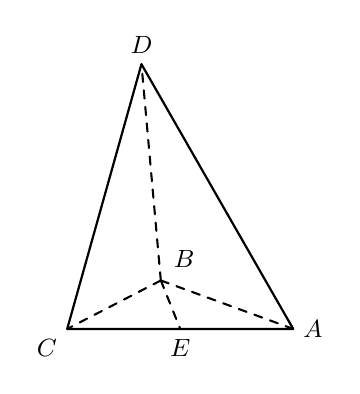
\begin{tikzpicture}[x=0.82cm,y=0.82cm,line cap=round,line join=round,line width=0.75pt,font=\small]
  \coordinate (A) at (3.5,0);
  \coordinate (B) at (1.45,0.75);
  \coordinate (C) at (0,0);
  \coordinate (D) at (1.15,4.1);
  \coordinate (E) at (1.75,0);
  \draw[thick] (C)--(D)--(A)--(C);
  \draw[dashed] (B)--(A) (B)--(C) (B)--(D) (B)--(E);
  \node[above] at (D) {$D$};
  \node[above right=1pt] at (B) {$B$};
  \node[below left] at (C) {$C$};
  \node[right] at (A) {$A$};
  \node[below] at (E) {$E$};
\end{tikzpicture}
\end{center}
\nopagebreak[4]
\Needspace{4\baselineskip}
\textbf{解析}

\Needspace{5\baselineskip}
令 $B=(0,0,0)$、$A=(2,0,0)$、$C=(0,2,0)$、$D=(0,0,d)$（$d>0$），则 $E=(1,1,0)$。取方向向量 $\overrightarrow{AD}=(-2,0,d)$、$\overrightarrow{BE}=(1,1,0)$，异面直线夹角满足

\nopagebreak[4]
\[
\frac{|\overrightarrow{AD}\cdot\overrightarrow{BE}|}
{|\overrightarrow{AD}|\,|\overrightarrow{BE}|}
=\frac{2}{\sqrt{4+d^2}\sqrt2}
=\frac{\sqrt{10}}{10}.
\]

\Needspace{5\baselineskip}
平方并化简得 $d^2=16$，故 $BD=4$。底面 $ABC$ 面积为 $\frac12\cdot2\cdot2=2$，于是

\nopagebreak[4]
\[
V=\frac13\cdot2\cdot4=\frac83.
\]

\gkanswer{答案：四面体体积为 $\dfrac83$。}

\end{answer}
\begin{answer}
\gksolhead{19}{}

\textbf{题目}：

\Needspace{5\baselineskip}
已知函数

\nopagebreak[4]
\[
f(x)=\dfrac{x^2+2x+a}{x},\quad x\in[1,+\infty).
\]

（1） 当 $a=\dfrac12$ 时，求函数 $f(x)$ 的最小值；

（2） 若对任意 $x\in[1,+\infty)$，$f(x)>0$ 恒成立，试求实数 $a$ 的取值范围。

\Needspace{4\baselineskip}
\textbf{解析}

改写为 $f(x)=x+2+a/x$。

\textbf{（1）} 当 $a=1/2$ 时，$f'(x)=1-1/(2x^2)>0$（$x\geq1$），故最小值在 $x=1$ 处取得，为 $7/2$。

\textbf{（2）} $x\geq1$，分母 $x$ 为正，只需 $x^2+2x+a>0$ 对所有 $x\geq1$ 成立。$x^2+2x$ 在区间上递增，最小值是 $3$，且在 $x=1$ 处取得，所以充要条件为 $3+a>0$，即 $a>-3$。

\gkanswer{答案（1）：$\dfrac72$，在 $x=1$ 处取得。}

\gkanswer{答案（2）：$a>-3$。}

\end{answer}
\begin{answer}
\gksolhead{20}{}

\textbf{题目}：

根据指令 $(r,\theta)$（$r\ge0$，$-180^\circ\le\theta\le180^\circ$），机器人在平面上能完成下列动作：先原地旋转角度 $\theta$（$\theta$ 为正时，按逆时针方向旋转 $\theta$；$\theta$ 为负时，按顺时针方向旋转 $-\theta$），再朝其面对的方向沿直线行走距离 $r$。

（1） 现机器人在直角坐标系的坐标原点，且面对 $x$ 轴正方向，试给机器人下一个指令，使其移动到点 $(4,4)$；

（2） 机器人在完成该指令后，发现在点 $(17,0)$ 处有一小球正向坐标原点作匀速直线滚动，已知小球滚动的速度为机器人直线行走速度的 2 倍，若忽略机器人原地旋转所需的时间，问机器人最快可在何处截住小球？并给出机器人截住小球所需的指令。（结果精确到小数点后两位）
\nopagebreak[4]
\begin{center}% Generator: hand-authored TikZ from the source-visible coordinate axes and printed ticks.
% Source: src-b46bf909434f6686413681f206c6f1c3566760d6e574f4799dc8b1e0658f9ee8
% PDF SHA-256: b798af61afdac624589769db5bbafe734aa9a0016973bd00b3f5bc8028ab3a40
% PDF page 2, printed page 71, question 20. No robot, ball, trajectory, or path is shown.
\begin{tikzpicture}[x=0.22cm,y=0.22cm,line cap=round,line join=round,line width=0.65pt,>=stealth,font=\small]
  \draw[->] (-1.4,0) -- (19.2,0) node[right] {$x$};
  \draw[->] (0,-1.2) -- (0,5.3) node[above] {$y$};
  \draw (4,-0.24) -- (4,0.24) node[below=3pt] {$4$};
  \draw (17,-0.24) -- (17,0.24) node[below=3pt] {$17$};
  \draw (-0.24,4) -- (0.24,4) node[left=3pt] {$4$};
  \node[below left] at (0,0) {$O$};
\end{tikzpicture}
\end{center}
\nopagebreak[4]
\Needspace{4\baselineskip}
\textbf{解析}

\textbf{（1）} 从原点到 $(4,4)$ 的距离为 $4\sqrt2$，方向角为 $45^\circ$，故可下达指令 $(4\sqrt2,45^\circ)$。完成后机器人朝向为 $45^\circ$。

\Needspace{5\baselineskip}
\textbf{（2）} 设机器人直线行走速度为 $v$，追截时已走距离为 $s$，则经过时间 $s/v$ 后，小球从 $(17,0)$ 向原点移动了 $2s$，位置为 $(17-2s,0)$。机器人从 $(4,4)$ 出发，故相遇需满足

\nopagebreak[4]
\[
(17-2s-4)^2+(0-4)^2=s^2,
\]

即 $3s^2-52s+185=0$，得 $s=5$ 或 $s=37/3$。最早相遇对应较小正根 $s=5$，小球位置为 $(7,0)$。从 $(4,4)$ 到该点的行进方向角为 $-\arctan(4/3)\approx-53.13^\circ$。机器人此时仍朝 $45^\circ$，所以指令转角为 $-53.13^\circ-45^\circ=-98.13^\circ$；指令为 $(5.00,-98.13^\circ)$。

\gkanswer{答案（1）：指令为 $(4\sqrt2,45^\circ)$。}

\gkanswer{答案（2）：最快在 $(7,0)$ 截住小球，所需指令为 $(5.00,-98.13^\circ)$。}

\end{answer}
\begin{answer}
\gksolhead{21}{}

\textbf{题目}：

\Needspace{5\baselineskip}
在 $xOy$ 平面上有一点列 $P_1(a_1,b_1)$、$P_2(a_2,b_2)$、$\cdots$、$P_n(a_n,b_n)$、$\cdots$，对每个自然数 $n$，点 $P_n$ 位于函数

\nopagebreak[4]
\[
y=2000\cdot\left(\dfrac{a}{10}\right)^2\quad(0<a<10)
\]

的图象上，且点 $P_n$、点 $(n,0)$ 与点 $(n+1,0)$ 构成一个以 $P_n$ 为顶点的等腰三角形。

（1） 求点 $P_n$ 的纵坐标 $b_n$ 的表达式；

（2） 若对每个自然数 $n$，以 $b_n$、$b_{n+1}$、$b_{n+2}$ 为边长能构成一个三角形，求 $a$ 取值范围；

（3） 设 $B_n=b_1b_2\cdots b_n$（$n\in\mathbb{N}$），若 $a$ 取（2）中确定的范围内的最小整数，求数列 $\{B_n\}$ 的最大项的项数。

\begin{gktip}
原页函数指数辨认为 2，本稿照录。该式与后续关于 $b_n$ 及 $B_n$ 的问法可能存在内容不一致；未据推理把指数改为 $n$，留待独立解题与同版材料复核。
\end{gktip}

\Needspace{4\baselineskip}
\textbf{解析}

题面函数指数按原页为 $2$，故按字面不含 $n$。又因 $P_n$ 是以 $(n,0)$、$(n+1,0)$ 为底边端点的等腰三角形顶点，必在垂直平分线 $x=n+1/2$ 上。因此 $a_n=n+1/2$，而原式给出共同纵坐标 $b_n=2000(a/10)^2=20a^2$。

\textbf{（1）} 在字面读法下，$b_n=20a^2$。

\textbf{（2）} 任意两腰长为 $\sqrt{(1/2)^2+(20a^2)^2}$，底边长为 $1$。因 $a>0$，腰长严格大于 $1/2$，故两腰之和大于底边，三角形不等式总成立；允许范围仍为 $0<a<10$。

\textbf{（3）} 该范围内最小整数 $a=1$，于是 $b_n=20$、$B_n=20^n$。该数列严格递增，没有最大项，因而题目按当前字面没有可给出的“最大项的项数”。在获得同版资料或可靠勘误以前，Q21 整体标记 \textbf{U/PENDING}，不以推测的指数替换原文。

\gkanswer{答案（1）：按原页指数 $2$ 的字面推导，$b_n=20a^2$。}

\gkanswer{答案（2）：$0<a<10$。}

\gkanswer{答案（3）：U/PENDING。}

\end{answer}
\begin{answer}
\gksolhead{22}{}

\textbf{题目}：

\Needspace{5\baselineskip}
已知复数 $z_0=1-mi$（$m>0$），$z=x+yi$ 和 $\omega=x'+y'i$，其中 $x$、$y$、$x'$、$y'$ 均为实数，$i$ 为虚数单位，且对于任意复数 $z$，有

\nopagebreak[4]
\[
\omega=\overline{z_0}\cdot\overline z,\quad |\omega|=2|z|\mbox{。}
\]

（1） 试求 $m$ 的值，并分别写出 $x'$ 和 $y'$ 用 $x$、$y$ 表示的关系式；

（2） 将 $(x,y)$ 作为点 $P$ 的坐标，$(x',y')$ 作为点 $Q$ 的坐标，上述关系可以看作是坐标平面上点的一个变换：它将平面上的点 $P$ 变到这一平面上的点 $Q$。当点 $P$ 在直线 $y=x+1$ 上移动时，试求点 $P$ 经该变换后得到的点 $Q$ 的轨迹方程；

（3） 是否存在这样的直线：它上面的任一点经上述变换后得到的点仍在该直线上？若存在，试求出所有这些直线；若不存在，则说明理由。

\begin{gktip}
文字层未可靠保留此处共轭线；经 PDF 第 2 页 300 dpi 局部放大，原页公式辨认为 $\omega=\overline{z_0}\cdot\overline z$，按原页录入。
\end{gktip}

\Needspace{4\baselineskip}
\textbf{解析}

\Needspace{5\baselineskip}
\textbf{（1）} $|\omega|=|z_0||z|=\sqrt{1+m^2}|z|=2|z|$，故 $m=\sqrt3$。由

\nopagebreak[4]
\[
\omega=\overline{z_0}\,\overline z
=(1+mi)(x-yi)
=(x+my)+i(mx-y)
\]

得 $x'=x+\sqrt3y$、$y'=\sqrt3x-y$。

\Needspace{5\baselineskip}
\textbf{（2）} 设 $P=(t,t+1)$，则

\nopagebreak[4]
\[
x'=(1+\sqrt3)t+\sqrt3,\qquad y'=(\sqrt3-1)t-1.
\]

消去 $t$，利用 $(\sqrt3-1)/(1+\sqrt3)=2-\sqrt3$，得到 $y'=(2-\sqrt3)x'+2-2\sqrt3$。

\Needspace{5\baselineskip}
\textbf{（3）} 设直线为 $y=kx+c$。线上点变换后满足

\nopagebreak[4]
\[
X=(1+\sqrt3k)x+\sqrt3c,\qquad Y=(\sqrt3-k)x-c.
\]

要求所有像点仍满足 $Y=kX+c$。比较 $x$ 的系数和常数项，得 $\sqrt3k^2+2k-\sqrt3=0$ 且 $(k\sqrt3+2)c=0$。

前式给 $k=1/\sqrt3$ 或 $k=-\sqrt3$；这两种情况下 $k\sqrt3+2$ 分别为 $3$ 和 $-1$，故都须 $c=0$。所有不变直线为 $y=x/\sqrt3$ 与 $y=-\sqrt3x$。

\gkanswer{答案（1）：$m=\sqrt3$，$x'=x+\sqrt3y$，$y'=\sqrt3x-y$。}

\gkanswer{答案（2）：$y'=(2-\sqrt3)x'+2-2\sqrt3$。}

\gkanswer{答案（3）：$y=\dfrac{x}{\sqrt3}$ 或 $y=-\sqrt3x$。}

\end{answer}